\documentclass[../dissertation.tex]{subfiles}

\begin{document}

\subsection{Experiment 7 - Vertical Scaling}
\label{experiment7-vertical-scaling}

Prior experiments have been setting the groundwork for these scaling experiments. It is now understood how a communication intensive ROS application behaves in the simple case (2 hosts, 2 nodes), and how switching to a wireless network affects the performance.

Now we wish to understand how adding more communication nodes will affect individual message latency, and total system throughput.

This experiment will involve adding more nodes to both sender, and echoer. Each sender node will send messages to 1 echoer node, who will echo the message back to that same sender node. This allows the sender to record both sent and receive times consistently.

More nodes will be added to each host, and message times recorded. The number of hosts will be a constant (2) as this experiment investigates the effect of increased nodes only.

The data used will be the sensor data stream used in previous experiments.

\subsubsection{Results}

Observations from the graphs:
- the Pi's cant support a "collective" total message throughput of greater than what we saw in the 2 node experiments (~350Hz)
- therefore we only see decent performance at 100Hz * 1 (sending) node, 100Hz * 2 nodes, 200Hz * 1 node, and 300Hz * 1 node.

\begin{figure}[H]
\centering
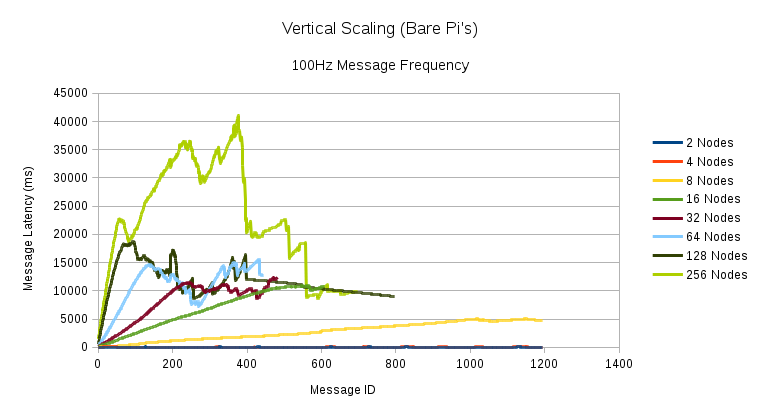
\includegraphics[width=\textwidth]{images/experiment7/vertical_scaling_100hz_all_freqs.png}
\caption{Experiment 7 - 100Hz Message Frequency, All Node Counts}
\label{exp7-100hz-allnodes}
\end{figure}

\begin{figure}[H]
\centering
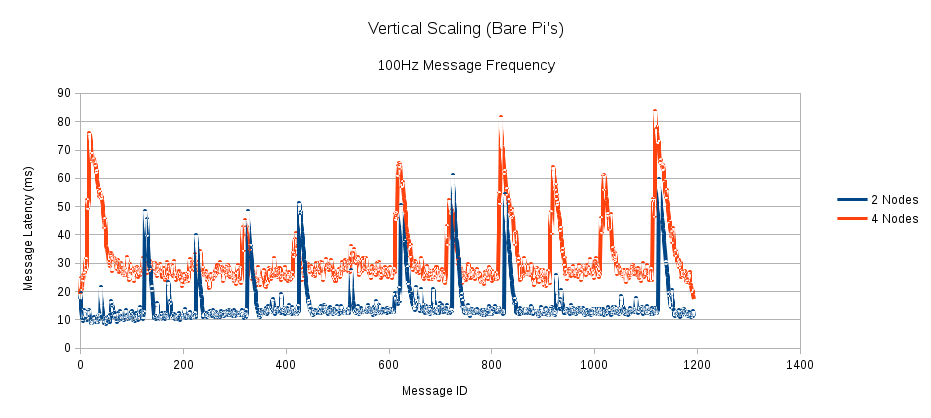
\includegraphics[width=\textwidth]{images/experiment7/vertical_scaling_100hz_low_freqs.png}
\caption{Experiment 7 - 100Hz Message Frequency, Low Node Counts}
\label{exp7-100hz-lownodes}
\end{figure}

\textit{A conclusion}

\end{document}
